\documentclass[11pt]{article}
\usepackage{ucs}
\usepackage[utf8x]{inputenc}
\usepackage{changepage}
\usepackage{graphicx}
\usepackage{amsmath}
\usepackage{gensymb}
\usepackage{amssymb}
\usepackage{enumerate}
\usepackage{tabularx}
\usepackage{lipsum}

\oddsidemargin 0.0in
\evensidemargin 0.0in
\textwidth 6.27in
\headheight 1.0in
\topmargin -0.1in
\headheight 0.0in
\headsep 0.0in
%\textheight 9.69in
\textheight 9.50in

\setlength\parindent{0pt}

\newenvironment{myenv}{\begin{adjustwidth}{0.4in}{0.4in}}{\end{adjustwidth}}
\renewcommand{\abstractname}{Anotācija}
\renewcommand\refname{Atsauces}

\newenvironment{uzdevums}[1][\unskip]{%
\vspace{3mm}
\noindent
\textbf{#1:}
\noindent}
{}

\newcommand{\subf}[2]{%
  {\small\begin{tabular}[t]{@{}c@{}}
  #1\\#2
  \end{tabular}}%
}



\newcounter{alphnum}
\newenvironment{alphlist}{\begin{list}{(\Alph{alphnum})}{\usecounter{alphnum}\setlength{\leftmargin}{2.5em}} \rm}{\end{list}}


\makeatletter
\let\saved@bibitem\@bibitem
\makeatother

\usepackage{bibentry}
%\usepackage{hyperref}


\begin{document}

\thispagestyle{empty}

{\Large \bf Ģeometriskas progresijas: Rudzātu vidusskola, 2019-07-31}

\begin{tabular}{@{}ll@{}} 
\begin{minipage}{0.61\columnwidth}
\begin{uzdevums}[1.jautājums]
Vienādsānu taisnleņķa trijstūrī $\triangle\,ABC$ ievilka kvadrātu tā, 
ka viena kvadrāta mala atrodas uz hipotenūzas $AB$, bet divas virsotnes uz atlikušajām malām. 
Virs šī kvadrāta tāpat ievilka nākamo kvadrātu, un tā tālāk.\\
Kādu daļu no sākotnējā trijstūra laukuma aizņem visu šo kvadrātu laukumu summa?
\end{uzdevums}
\end{minipage} &
\begin{minipage}{0.39\columnwidth}
\begin{center}
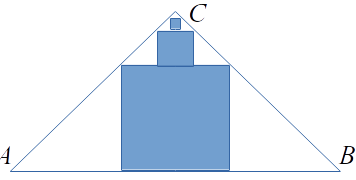
\includegraphics[width=2.00in]{triangles.png}
\end{center}
\end{minipage}
\end{tabular}

\vspace{2ex}
{\em Ierakstiet laukumu attiecību:} \_\_\_\_\_\_\_\_\_\_\_\_\_\_\_


\vspace{6ex}
\begin{uzdevums}[2.jautājums]
Pārveidot par parastiem daļskaitļiem (izteikt formā $P/Q$):\\
{\bf (a)} $0.27272727\ldots=0.(27)$
{\bf (b)}  $0.123123123\ldots=0.(123)$
{\bf (c)}  $0.041666666\ldots=0.041(6)$
\end{uzdevums}

\vspace{2ex}
{\em (a) $0.(27)=$} \_\_\_\_\_ 
{\em (b) $0.(123)=$} \_\_\_\_\_
{\em (c) $0.041(6)=$} \_\_\_\_\_


\vspace{6ex}
\begin{uzdevums}[3.jautājums]
Daļskaitļa $x \in [0,1]$ pieraksts {\em divnieku skaitīšanas sistēmā}
ir bezgalīga virkne $0,d_1d_2d_3\ldots$, kur $d_1,d_2,\ldots$ pieņem vērtības
$0$ vai $1$, bet $x$ izsakāms kā bezgalīga summa: 
$$x = \frac{d_1}{2^1} + \frac{d_2}{2^2} + \frac{d_3}{2^3} + \ldots$$
Atrast pirmos $10$ ciparus aiz komata skaitļa ${\displaystyle \frac{3}{7}}$ divnieku pierakstā. 
\end{uzdevums}

\vspace{2ex}
{\em Ierakstiet $\frac{3}{7}$ divnieku pierakstā pirmos desmit ciparus:} $0,$\_\_\_\_\_\_\_\_\_\_


\vspace{6ex}
\begin{uzdevums}[4.jautājums]
Kāds atlikums rodas, ja skaitli $N=2^{15}-1$ dala ar $2^5-1$? Un ar $2^6-1$? 
\end{uzdevums}

\vspace{2ex}
{\em Ierakstiet atlikumu, ja $N$ dala ar $2^5-1$:} \_\_\_\_\_

\noindent
{\em Ierakstiet atlikumu, ja $N$ dala ar $2^6-1$:} \_\_\_\_\_

\vspace{6ex}
\begin{uzdevums}[5.jautājums]
Atrast šo 11 skaitļu ģeometrisko vidējo: $1, \frac{3}{2}, \left( \frac{3}{2} \right)^2, \left( \frac{3}{2} \right)^3, \ldots, \left( \frac{3}{2} \right)^{10}$.\\
{\em Piezīme.} Par skaitļu $a_1,a_2,\ldots,a_n$ ģeometrisko vidējo, ja visi $a_i \geq 0$, sauc skaitli 
$m = \sqrt[n]{a_1\cdot{}a_2\cdot\ldots\cdot{}a_n}$. 
\end{uzdevums}

\vspace{2ex}
{\em Ierakstiet ģeometrisko vidējo kā $P/Q$ vai vienkāršotu sakņu izteiksmi:} \_\_\_\_\_

\end{document}
